\chapter{Computación en \ac{GPU} con CUDA y pycuda}
\label{cap:computacion}

\begin{resumen}
	En este capítulo se pretenden introducir los conceptos básicos de la programación en \ac{GPU}, en particular en el lenguaje CUDA C++ utilizado desde la librería de Python pycuda.
\end{resumen}


\section{Bases de la programación en \ac{GPU}}
Las \ac{GPU}s son componentes hardware del ordenador pensados para acelerar el procesamiento de los gráficos. Esto se hace aprovechando que la mayoría de los cómputos que se requieren para procesar estos se puede ejecutar de manera simultánea en paralelo.

Dada la naturaleza de las tarjetas gráficas, resulta natural el utilizarlas para implementar algoritmos que puedan beneficiarse de este paralelismo. Con ese fin, NVIDIA desarrolló el lenguage de programación \ac{CUDA}\footnote{Puede consultarse el manual completo de \ac{CUDA} en este \href{https://docs.nvidia.com/cuda/pdf/CUDA_C_Programming_Guide.pdf}{\emph{enlace}}}, una extensión de C/C++ que permite la definición de \emph{kernels}. 

Los \emph{kernels} son funciones de C/C++ diseñadas para ejecutarse en varios hilos al mismo tiempo en la \ac{GPU} (a la que llamaremos \emph{dispositivo} en este contexto). Estos kernels serán luego ejecutados desde la \ac{CPU}, que en este contexto llamaremos \emph{host}.



\section{Programación en pycuda}
Como adelantamos en la Sección \ref{cap:introduccion}, utilizaremos pycuda para poder ejecutar código \ac{CUDA} en la GPU desde un programa convencional en Python. Este será el proceso para hacer un programa:

\begin{enumerate}
	\item Generar archivos con la extensión .cu que contengan la definición de las funciones que vayamos a ejecutar en la GPU, escritas en \ac{CUDA}. Este será el único código que escribamos en este lenguaje de programación, todo lo demás estará escrito en Python.
	\item Crear un programa en Python, que será el que ejecutemos. Éste será el que se encargue de compilar y llamar (mediante las funciones de pycuda) a las funciones definidas en el apartado anterior. Para hacer esto, utilizaremos el programa generateMod.py (ver \ref{code:generateMod}). Además del programa como tal, tendremos que utilizar unas funciones de pycuda para reservar memoria y llevar los datos al dispositivo (para ver más sobre la gestión de memoria en dispositivo, ver \ref{subsec:gestionDeMemoria}).
\end{enumerate}




\section{Programación en \ac{CUDA}}
Aunque no vayamos a escribir mucho código en este lenguaje propiamente, necesitamos entender bien cómo funciona para evitar errores.
La única diferencia que nos encontramos con C/C++ en la sintaxis, es que todos los \textit{kernels} que definamos tienen que tener uno de los siguientes identificadores, que describe desde dónde se van a llamar y dónde se van a ejecutar:
\begin{description}
	\item[device] Funciones que van a ser llamadas y ejecutadas desde el dispositivo (la \ac{GPU})
	\item[global] Funciones que van a se llamadas desde la \ac{CPU} pero ejecutadas en el dispositivo. Cuando llamemos a estas funciones les pasaremos como meta-parámetro el número de veces que se van a ejecutar.
	\item[host] Son funciones habituales de C++. Dado que vamos a utilizar \ac{CUDA} a través de pycuda, no utilizaremos este tipo de funciones, ya que toda la programación en CPU la haremos en Python.
\end{description}
\subsection{Gestión de memoria}
\label{subsec:gestionDeMemoria}
Es importante comprender que el dispositivo y el host son unidades de computación diferentes. Esto significa que no comparten espacio de direcciones de memoria y, por tanto, tenemos que proceder de manera distinta dependiendo si estamos usando variables del dispositivo o del host.

A pesar de la necesidad de entender el funcionamiento de la memoria, no usaremos las funciones de  gestión de memoria de CUDA, ya que la librería pycuda tiene sus propias funciones para hacer esto de manera un poco más cómoda.
\subsubsection{Memoria en el host}
Para trabajar con la memoria en la \ac{CPU} se utilizarían las funciones habituales de C/C++ como \emph{malloc} (para reservar memoria), pero como estamos trabajando sobre Python, no tenemos que preocuparnos por eso.
\subsubsection{Memoria en el dispositivo}
Al crear la memoria para el dispositivo desde el host, no podemos emplear las funciones habituales, pues estas no reservan memoria en la \ac{GPU}. Existen funciones específicas para esto como \emph{cudaMalloc}.
\subsubsection{Compartir memoria entre dispositivo y host}
Para esto, usamos unas funciones que nos proporciona pycuda, \emph{memcpy\_htod} y \emph{memcpy\_dtoh}, que nos permiten copiar memoria desde el host al dispositivo y en dirección contraria respectivamente.

\subsection{Hilos y bloques}
Al ejecutar un kernel, tenemos que especificar cuantos hilos ejecutarán esa función, los hilos se organizan en bloques, que a su vez se organizan en una cuadrícula (grid)\footnote{En las últimas versiones también podemos tener Thread Block Clusters para agrupar bloques, pero esos no los trataremos en este trabajo.} como podemos observar en la imagen \ref{fig:grid}


\begin{figure}
	\centering
	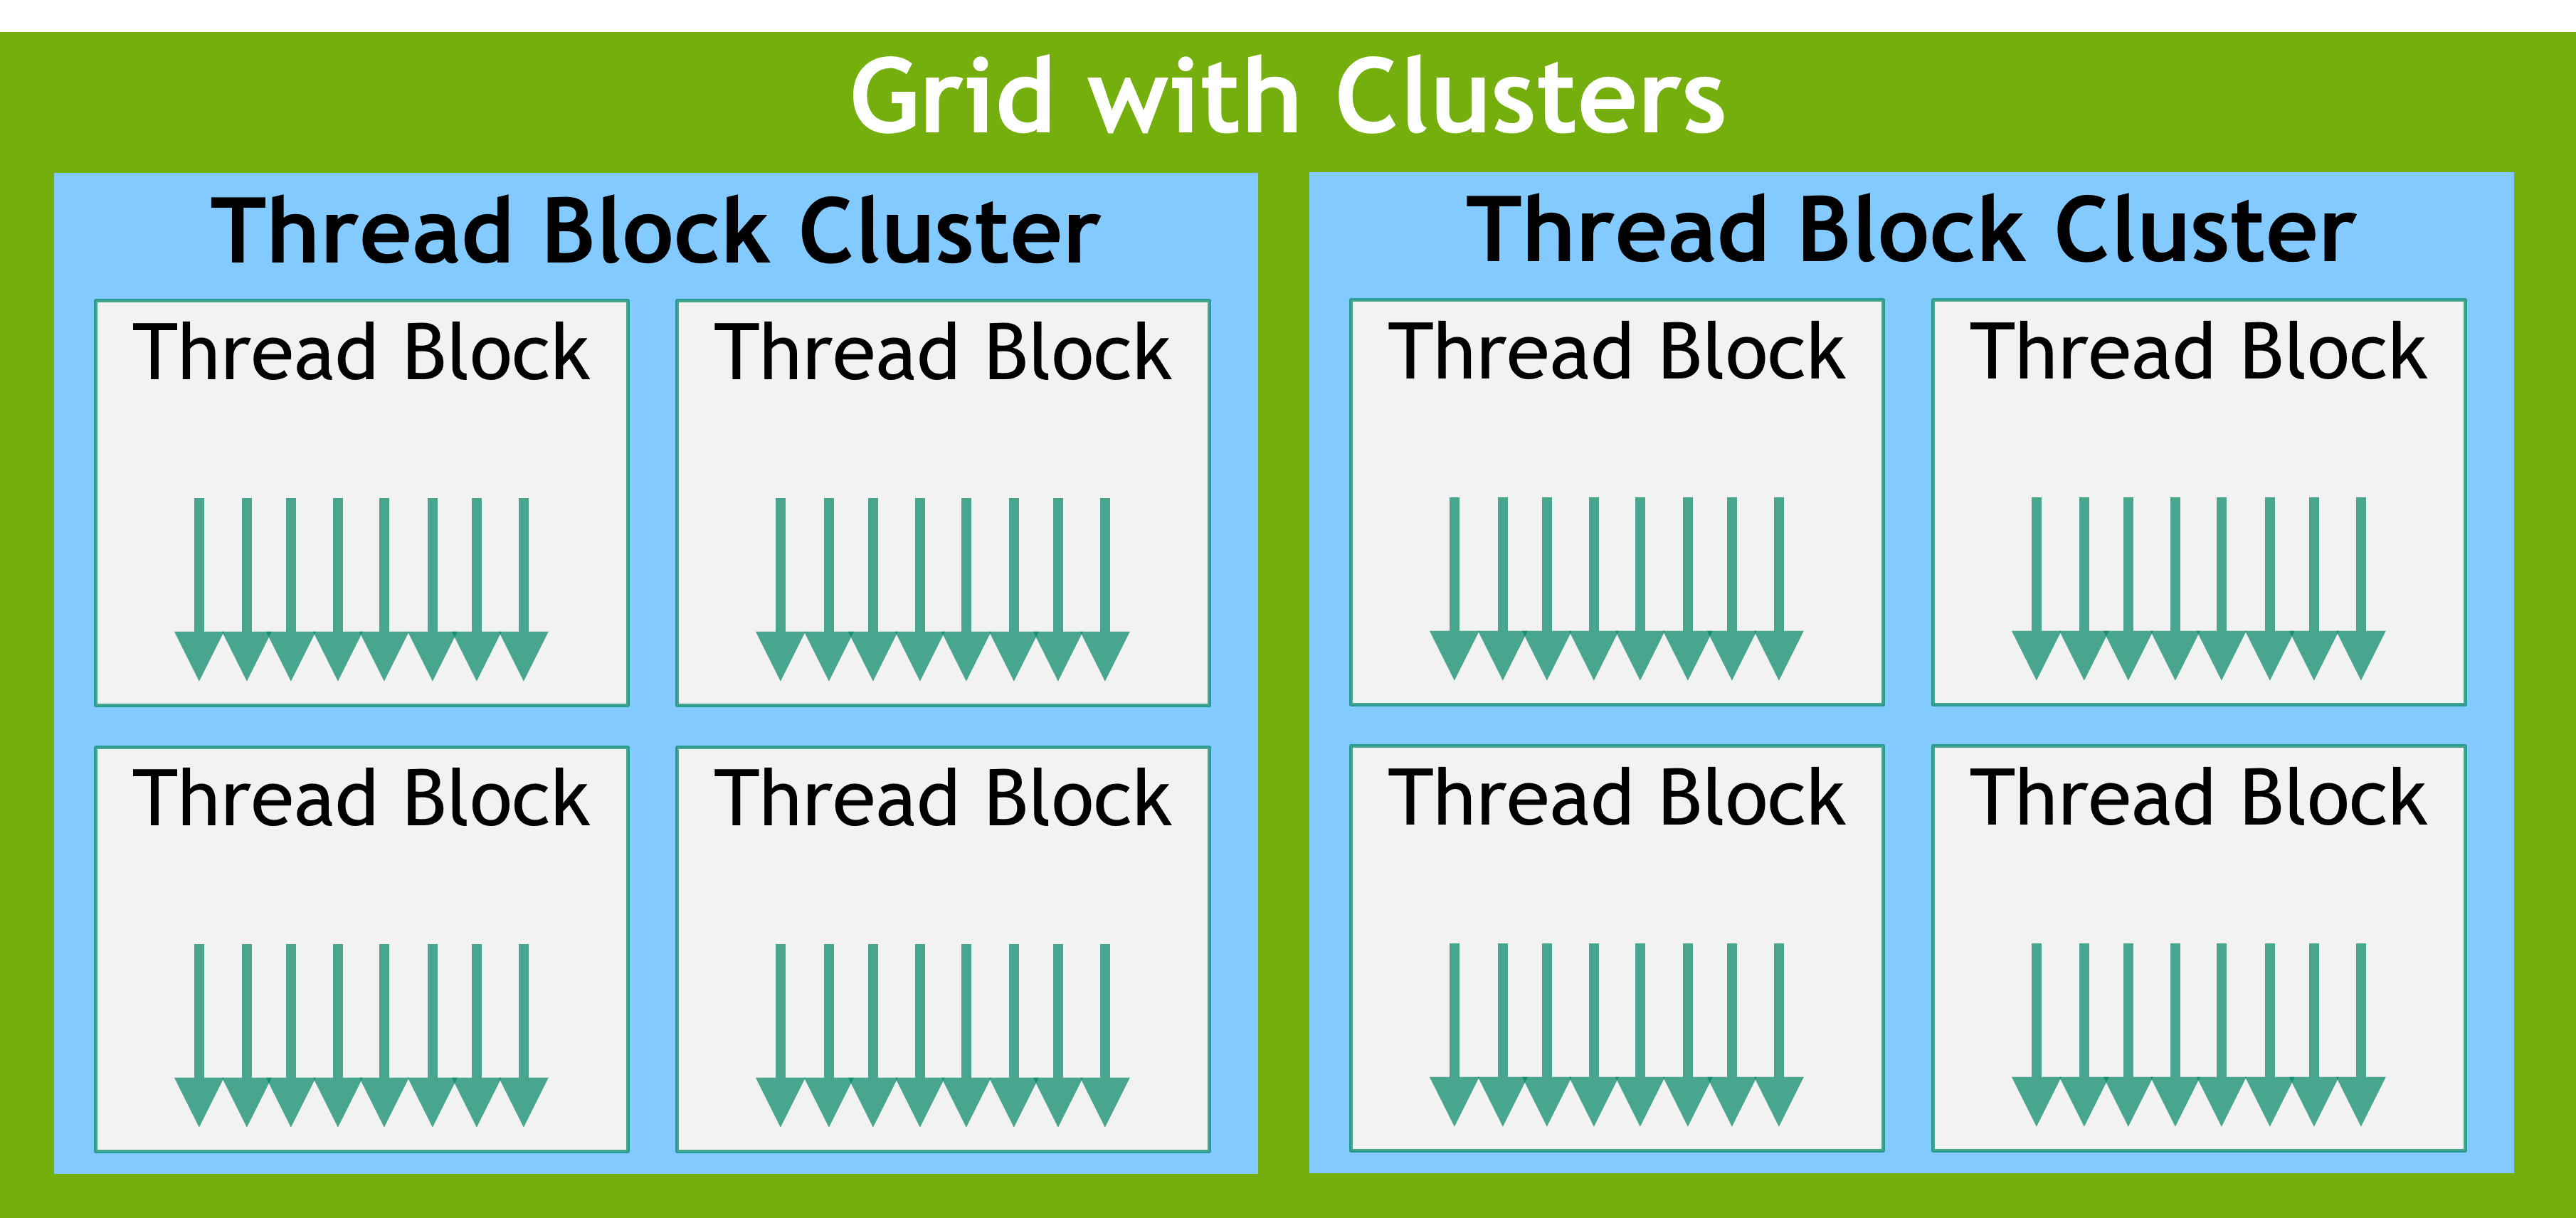
\includegraphics[width=0.7\linewidth]{Imagenes/Bitmap/grid}
	\caption{Cuadrícula de bloques de hilos}
	\label{fig:grid}
\end{figure}


Un bloque es un conjunto de hilos (que se distribuyen en tres dimensiones) que, como máximo, puede tener 1024 hilos diferentes por motivos de implementación en memoria (podemos tener un bloque de 1024x1x1 o 256x2x2 por ejemplo, pero no de 256x4x2, ya que el límite se refiere a la cantidad total de hilos, no al máximo en cada dimensión).

Podemos tener tantos bloques como queramos, organizados a su vez en la cuadrícula (también tridimensional). En cada hilo podemos acceder al índice de su bloque y del hilo dentro del bloque con \emph{blockIdx.dim} y \emph{threadIdx.dim} respectivamente, siendo dim la dimensión, osea x, y o z.

Aunque a nivel de usuario pueda parecer enrevesada esta distribución, esto está estrechamente relacionado con la implementación y la memoria compartida como podemos observar en la imagen \ref{fig:mem}. Todos los hilos tienen su propia memoria privada y una memoria compartida entre los demás hilos de su bloque, pero para compartir memoria con otros bloques hay que utilizar otros mecanismos que pueden afectar al rendimiento, luego implementar los hilos de manera adecuada puede hacer más eficientes los programas.

\begin{figure}
	\centering
	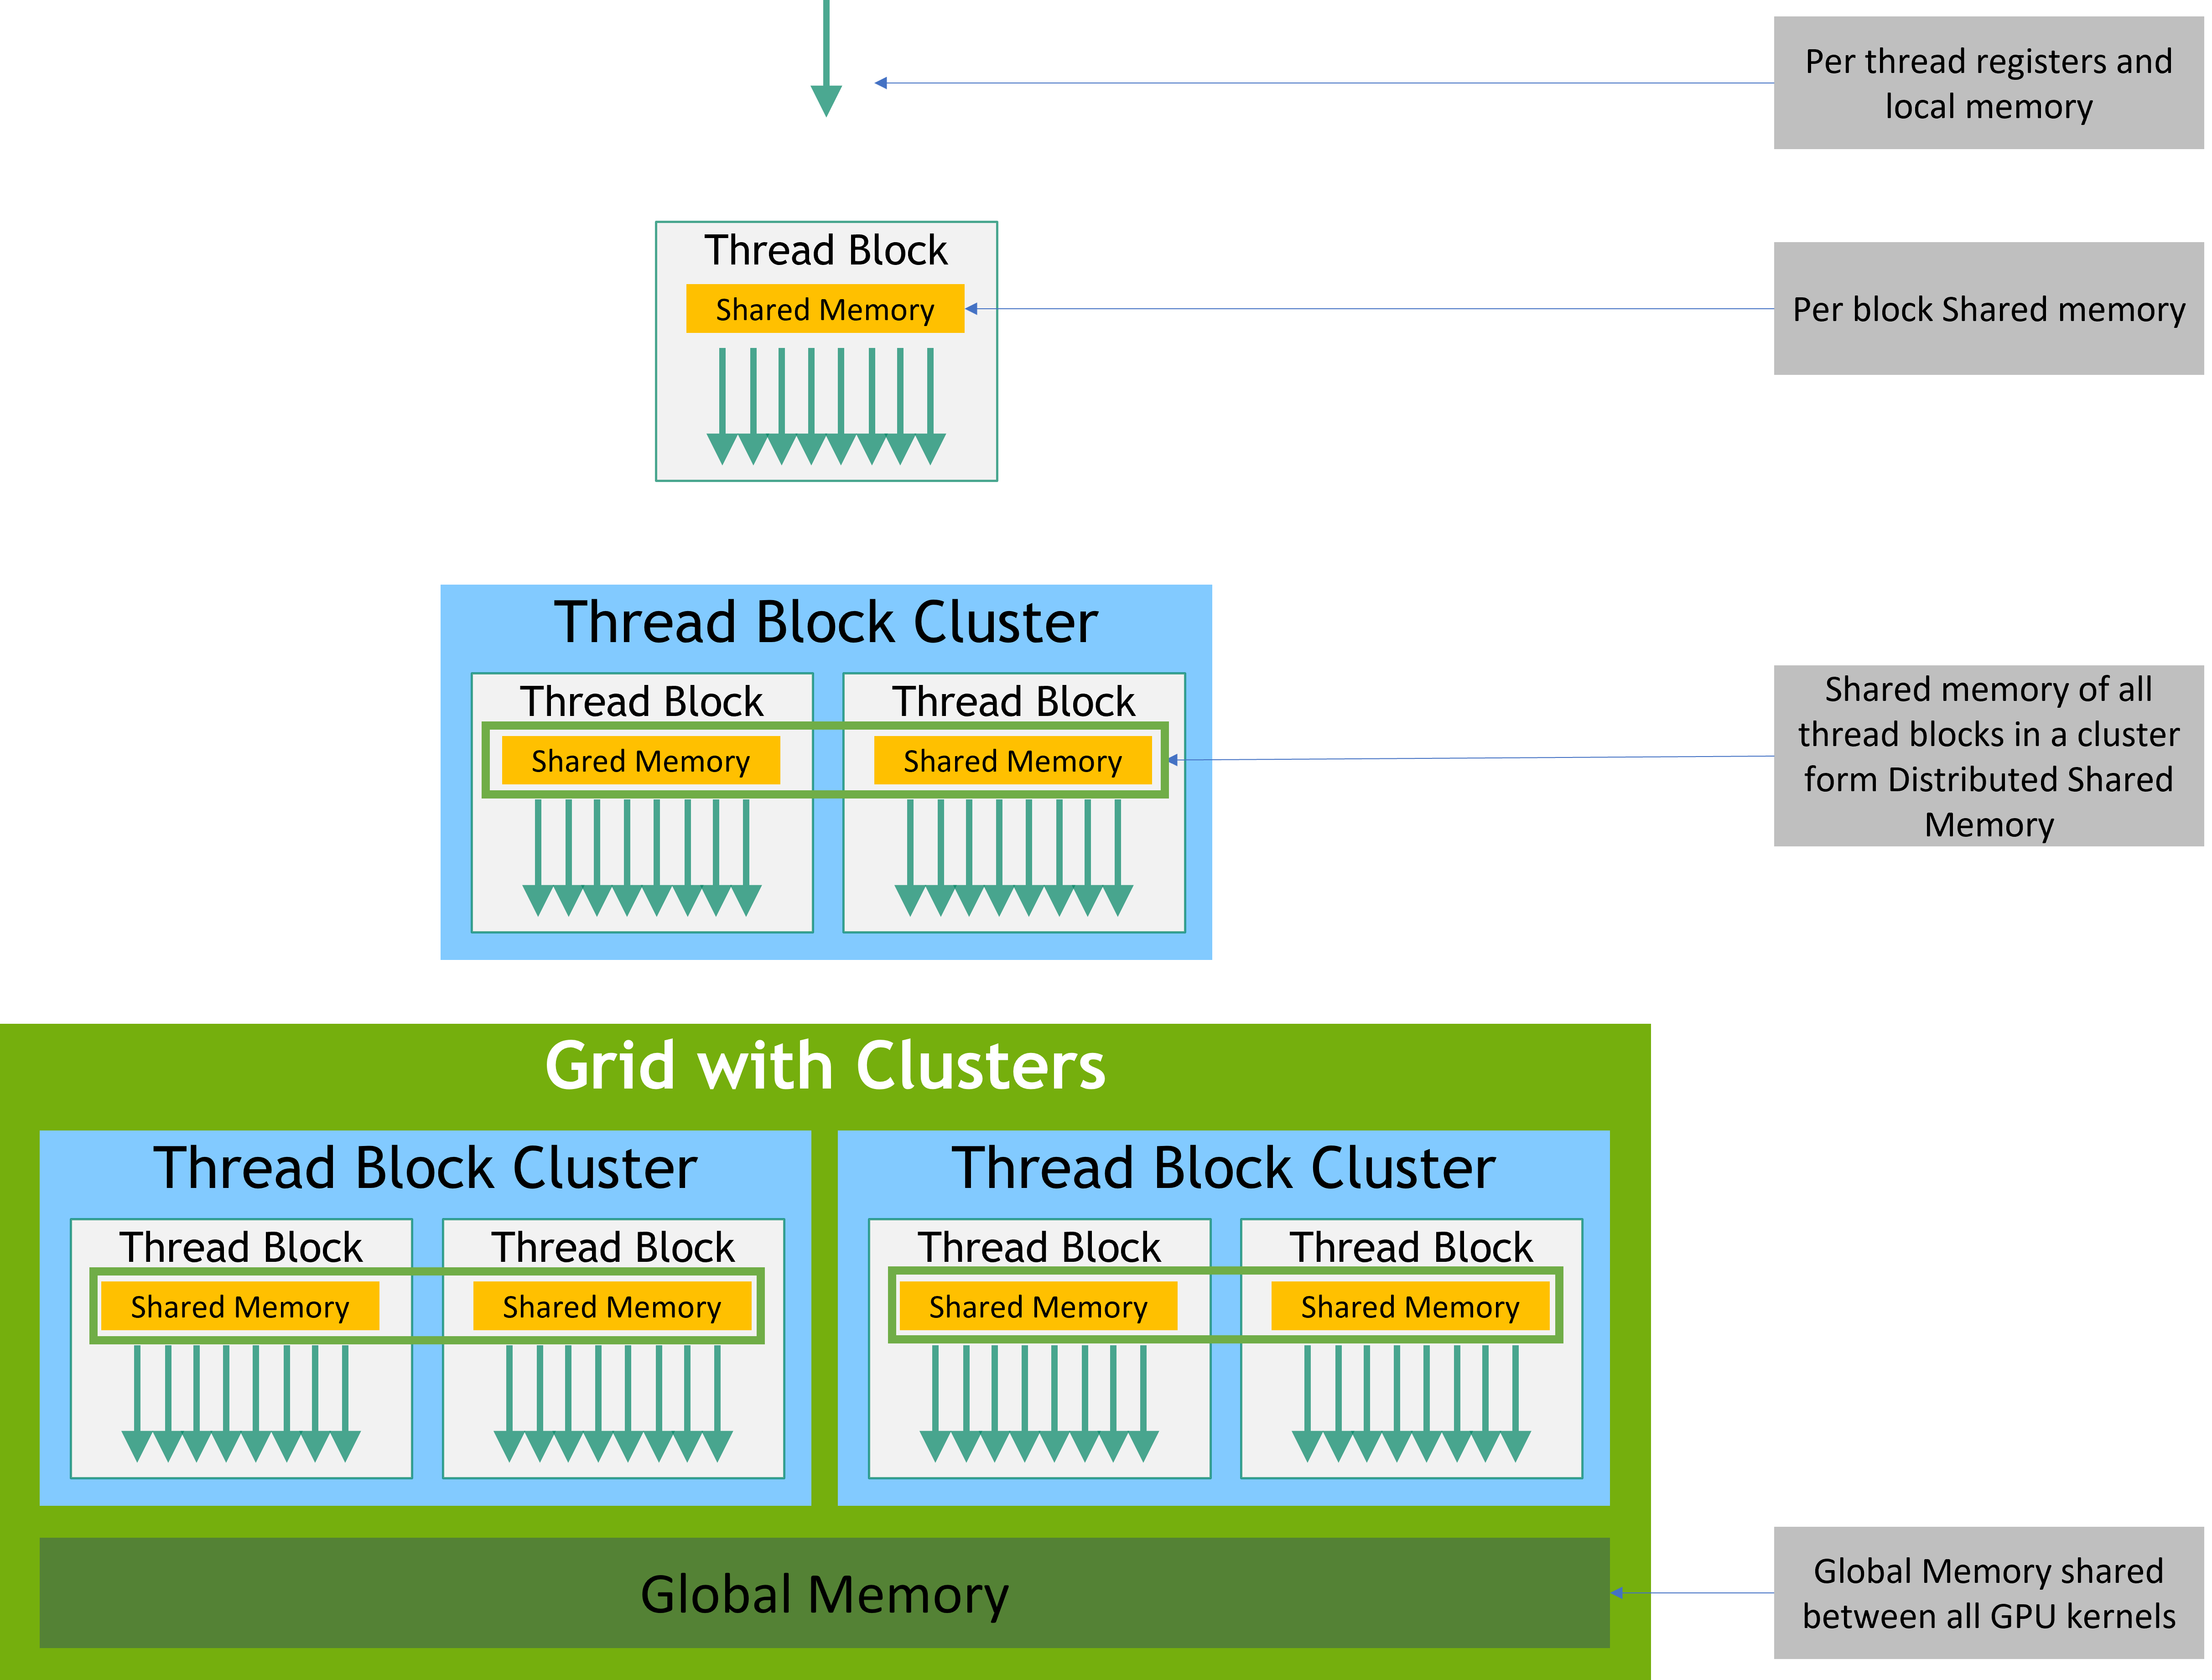
\includegraphics[width=0.7\linewidth]{Imagenes/Bitmap/memory}
	\caption{Memoria compartida entre elementos}
	\label{fig:mem}
\end{figure}


\section{Ejemplos}
Procedemos ahora a hacer un par de ejemplos sencillos que nos permitan familiarizarnos con estos conceptos.

\subsection{Hola Mundo}
Como es costumbre a la hora de programar, lo primero es hacer un "hola mundo", un programa que escriba en la consola la frase "hola mundo". Como el objetivo es poner de manifiesto que las cosas se están ejecutando varias veces en la \ac{GPU}, escribiremos el texto dos veces.

$\bullet$ En \ref{code:HelloWorldPY} vemos un ejemplo de uso de \textit{generateMod.py}, así como las funciones para reservar y copiar memoria en pycuda. Es importante destacar que a la hora de llamar al kernel desde la CPU, le tenemos que indicar qué forma va a tener cada uno de los bloques (osea, el número de hilos y cómo van a estar repartidos a lo largo de sus dimensiones).

$\bullet$ En \ref{code:HelloWorldCU} podemos ver la implementación del hola mundo en \ac{CUDA}, con el uso de la etiqueta \textbf{\_\_global\_\_} mencionada anteriormente.

$\bullet$ En \ref{code:HelloWorldOUT} vemos que la salida es la esperada.

\subsection{Suma de vectores}
Habiendo tenido ya nuestro primer contacto con pycuda, vamos ahora a poner de manifiesto la mejora de rendimiento que se puede conseguir. Vamos a realizar la suma de dos vectores de tamaños incrementalmente grandes, primero en CPU y luego en GPU, y vamos a comparar los tiempos que tarda en hacer ambas cosas.

$\bullet$ En \ref{code:vectorAddPY} podemos ver un ejemplo más complejo de código Python usando pycuda. La función \textit{add\_random\_vects} genera dos vectores de números aleatorios y los suma, primero en la CPU, y luego en GPU, midiendo el tiempo de ambos. Hay que destacar un par de cosas importantes:

Por un lado, hay que hacer la gestión de memoria, osea reservar memoria en GPU y copiar los datos con las funciones de pycuda. Por otro lado hay que gestionar el tamaño de bloque. Recordemos que los bloques pueden tener a lo sumo 1024 hilos, mientras que las grids pueden ser arbitrariamente grandes\footnote{En realidad hay un límite de tamaño dependiente del hardware, pero es tan grande que puede desestimarse}, esto implica que podríamos simplemente ejecutar un hilo por bloque y tantas mallas como el tamaño del vector, pero si recordamos la imagen \ref{fig:mem} podemos observar que los hilos de cada bloque comparten memoria local, por lo que si hacemos el máximo uso posible de los bloques (osea tratar con bloques de 1024 hilos), haremos un menor uso de la memoria y, por tanto, obtendremos resultados notablemente mejores.

Por último, comprobamos que las sumas coincidan y mostramos el incremento de eficiencia. Al ejecutar este script, simplemente llamamos a la función para valores de n entre $1$ y $10^{10}$

$\bullet$ En \ref{code:vectorAddCU} el código es bastante inmediato, calculamos el índice al que le corresponde nuestro hilo concreto y hacemos la suma. Solo hay una sutileza, y es que, en el último bloque que utilicemos, probablemente algunos hilos estén trabajando posiciones no válidas (porque todos los bloques tienen la misma cantidad de hilos, luego hay más hilos que posiciones en el vector). Para no acceder a posiciones de memoria posiblemente inválidas, simplemente añadimos a los datos de entrada el tamaño del vector y, si el hilo tiene un índice superior al tamaño del vector, no hacemos nada.

$\bullet$ En \ref{code:vectorAddOUT} se pone de manifiesto la mejora en la eficiencia, y es que cuando el tamaño del vector es suficientemente grande, el algoritmo es unas 10 veces más rápido. 




